% !TeX program = lualatex

\documentclass[
	ngerman,
	ruledheaders=section,%Ebene bis zu der die Überschriften mit Linien abgetrennt werden, vgl. DEMO-TUDaPub
	class=report,% Basisdokumentenklasse. Wählt die Korrespondierende KOMA-Script Klasse
	thesis={type=bachelor},% Dokumententyp Thesis, für Dissertationen siehe die Demo-Datei DEMO-TUDaPhd
	accentcolor=9c,% Auswahl der Akzentfarbe
	custommargins=false,% Ränder werden mithilfe von typearea automatisch berechnet
	marginpar=false,% Kopfzeile und Fußzeile erstrecken sich nicht über die Randnotizspalte
	%BCOR=5mm,%Bindekorrektur, falls notwendig
	parskip=half-,%Absatzkennzeichnung durch Abstand vgl. KOMA-Script
	fontsize=11pt,%Basisschriftgröße laut Corporate Design ist mit 9pt häufig zu klein
%	logofile=example-image, %Falls die Logo Dateien nicht vorliegen
]{tudapub}


% Der folgende Block ist nur bei pdfTeX auf Versionen vor April 2018 notwendig
\usepackage{iftex}
\ifPDFTeX
	\usepackage[utf8]{inputenc}%kompatibilität mit TeX Versionen vor April 2018
\fi

%%%%%%%%%%%%%%%%%%%
%Sprachanpassung & Verbesserte Trennregeln
%%%%%%%%%%%%%%%%%%%
\usepackage[ngerman, main=english]{babel}
\usepackage[autostyle]{csquotes}% Anführungszeichen vereinfacht
\usepackage{microtype}

%%%%%%%%%%%%%%%%%%%
%Literaturverzeichnis
%%%%%%%%%%%%%%%%%%%
%\usepackage{biblatex}   % Literaturverzeichnis
\usepackage[backend=biber,style=numeric,sorting=none]{biblatex}

\addbibresource{BibTexDatei.bib}

%%%%%%%%%%%%%%%%%%%
%Paketvorschläge Tabellen
%%%%%%%%%%%%%%%%%%%
%\usepackage{array}     % Basispaket für Tabellenkonfiguration, wird von den folgenden automatisch geladen
\usepackage{tabularx}   % Tabellen, die sich automatisch der Breite anpassen
%\usepackage{longtable} % Mehrseitige Tabellen
%\usepackage{xltabular} % Mehrseitige Tabellen mit anpassarer Breite
\usepackage{booktabs}   % Verbesserte Möglichkeiten für Tabellenlayout über horizontale Linien

%%%%%%%%%%%%%%%%%%%
%Paketvorschläge Mathematik
%%%%%%%%%%%%%%%%%%%
%\usepackage{mathtools} % erweiterte Fassung von amsmath
%\usepackage{amssymb}   % erweiterter Zeichensatz
%\usepackage{siunitx}   % Einheiten

%Formatierungen für Beispiele in diesem Dokument. Im Allgemeinen nicht notwendig!
\let\file\texttt
\let\code\texttt
\let\tbs\textbackslash

\usepackage{pifont}% Zapf-Dingbats Symbole
\newcommand*{\FeatureTrue}{\ding{52}}
\newcommand*{\FeatureFalse}{\ding{56}}

\begin{document}

\Metadata{
	title= Concepts for operating ground based rescue robots using virtual reality,
	author=Jingyi Jia
}

\title{Concepts for operating ground based rescue robots using virtual reality}
%\subtitle{\LaTeX{} using TU Darmstadt's Corporate Design}
\author{Jingyi Jia}%optionales Argument ist die Signatur,
\birthplace{Shanghai, China}%Geburtsort, bei Dissertationen zwingend notwendig
\reviewer{Prof. Dr. Max Mühlhäuser \and Julius von Willich}%Gutachter


\department{inf} % Das Kürzel wird automatisch ersetzt und als Studienfach gewählt, siehe Liste der Kürzel im Dokument.
\institute{Telekooperation}
\group{Prof. Dr. Max Mühlhäuser}

\submissiondate{\today}
\examdate{\today}


\maketitle
\affidavit
\tableofcontents

\chapter{Abstract}

\chapter{Introduction}
In recent years, natural disasters such as earthquakes, tsunamis and potential nuclear, chemical, biological and explosives have seriously threatened the safety of human life and property. While the number of various disasters has increased, their severity, diversity and complexity have also gradually increased. The 72h after a disaster is the golden rescue time, but the unstructured environment of the disaster site makes it difficult for rescuers to work quickly, efficiently and safely.

Rescue robots have the advantages of high mobility and handling breaking capacity, can work continuously to improve the efficiency of search and rescue, and can achieve the detection of graph, sound, gas and temperature within the ruins by carrying a variety of sensors, etc.
Moreover, the robot rescue can assist or replace the rescuers to avoid the injuries caused by the secondary collapse and reduce the risk of rescuers. Therefore, rescue robots have become an important development direction.

In fact, rescue robots have been put to use in a number of disaster scenarios. The Center for Robot-Assisted Search and Rescue (CRASAR) used rescue robots for Urban Search and Rescue (USAR) task during the World Trade Center collapse in 2001 \cite{Casper:2003tk} and has employed rescue robots at multiple disaster sites in the years since to assist in finding survivors, inspecting buildings and scouting the site environment etc \cite{Murphy:2012th}. Anchor Diver III was utilized as underwater support to search for bodies drowned at sea after the 2011 Tohoku Earthquake and Tsunami \cite{Huang:2011wq}.

Considering the training time and space constraints for rescuers \cite{Murphy:2004wl}, and the goal of efficiency and fluency collaboration \cite{10.1145/1228716.1228718}, the appropriate human-robot interaction approach deserves to be investigated. Some of the existing human-computer interaction methods are Android software \cite{Sarkar:2017tt} \cite{Faisal:2019uu}, gesture recognition\cite{Sousa:2017tn} \cite{10.1145/2157689.2157818} \cite{Nagi:2014vu}, facial voice recognition \cite{Pourmehr:2013ta}, adopting eye movements \cite{Ma:2015wu}, Augmented Reality(AR)\cite{SOARES20151656} and Virtual Reality(VR), etc.
\chapter{Related Work}
\label{related}

In this chapter, some research on the integration of \gls{vr} and \gls{hri} will be discussed. The relevant literature and its contributions will be briefly presented. 

The topic of \gls{vr} and \gls{hri} is an open research topic with many kinds of focus perspectives.

\gls{hri} platforms combined with virtual worlds have many applications. It can be used, for example, to train machine operators in factories. Elias Matsas et al. \cite{Matsas:2017aa} provided a \gls{vr}-based training system using hand recognition. Kinect cameras are used to capture the user's positions and motions, and virtual user models are constructed in the \gls{vr} environment based on the collected data. Users will operate robots and virtual objects in the \gls{vr} environment, and in this way, learn how to operate the real robot. The framework proposed by Luis Pérez et al. \cite{Perez:2019ub} is applied to train operators to learn to control the robot. Since the environment does not need to change in real time, but rather needs to recreate the factory scene realistically, a highly accurate 3D environment was constructed in advance using Blender in combination with a 3D scanner.

Building 3D scenes in virtual worlds based on information collected by robots is also a research highlight. Wang, et al. \cite{Wang:2017uy} were concerned with the visualization of the rescue robot and its surroundings in a virtual environment. The proposed \gls{hri} system uses the incremental 3D-NDT map to render the robot's surroundings in real time. The user can view the robot's surroundings in a first-person view through the \gls{htc} and send control commands through arrow keys on the motion controllers. A novel \gls{vr}-based practical system is presented in \cite{Stotko:2019ud} consisting of distributed systems to reconstruct the 3D scene. The data collected by the robot is first transmitted to the client responsible for reconstructing the scene. After the client has constructed the 3D scene, the set of actively reconstructed visible voxel blocks is sent to the server responsible for communication, which has a robot-based live telepresence and teleoperation system. This server will then broadcast the data back to the client used by the operator, thus enabling an immersive visualization of the robot within the scene.

Others are more concerned about the manipulation of the robotic arm mounted on the robot. Moniri et al. \cite{Moniri:2016ud} provided a \gls{vr}-based operating model for the robotic arm. The user wearing a headset can see a simulated 3D scene at the robot's end and send pickup commands to the remote robot by clicking on the target object with the mouse. The system proposed by Ostanin et al. \cite{Ostanin:2020uo} is also worth mentioning. Although their proposed system for operating a robotic arm is based on \gls{mr}, the article is highly relevant to this thesis, considering the correlation of \gls{mr} and \gls{vr} and the proposed system detailing the combination of \gls{ros} and robotics. In their system, \gls{ros} Kinect is used as middleware and responsible for communicating with the robot and the \gls{unity} side. The user can control the movement of the robot arm by selecting predefined options in the menu. In addition, the orbit and target points of the robot arm can be set by clicking on a hologram with a series of control points.

%Summary
To summarize, previous work has studied methods and tools for \gls{vr}-based \gls{hri} and teleoperation. However, only few studies focus on the different interactive approaches for \gls{hri}.
\chapter{Implementation}
\label{implementation}

% summary
In this chapter, the tools and techniques used in building this human-computer collaborative VR-based system are described. The focus will be on interaction techniques for different modes of operation. In addition, the setup of the robot and the construction of test scenes will also be covered in this chapter.


\section{Overview}
The main goal of this work is to design and implement a VR-based human-robot collaboration system with different methods of operating the robot in order to find out which method of operation is more suitable to be used to control the rescue robot. Further, it is to provide some basic insights for future development directions and to provide a general direction for finding an intuitive, easy-to-use and efficient operation method. Therefore, the proposed system was developed using Unity, including four modes of operation and a corresponding test environment for simulating post-disaster scenarios. In each operation mode, the user has a different method to control the robot. In addition, in order to better simulate the process by which the robot scans its surroundings and the computer side cumulatively gets a reconstructed 3D virtual scene, the test environment was implemented in such a way that the picture seen by the user depends on the direction of the robot's movement and the trajectory it travels through.


\section{System Architecture}
The proposed system runs on a computer with the Windows 10 operating system. This computer has been equipped with an Intel Core i7-8700K CPU, 32 GB RAM as well as a NVIDIA GTX 1080 GPU with 8 GB VRAM. HTC Vive is used as a VR device. It has a resolution of 1080 × 1200 per eye, resulting in a total resolution of 2160 × 1200 pixels, a refresh rate of 90 Hz, and a field of view of 110 degrees. It includes two motion controllers and uses two Lighthouses to track the position of the headset as well as the motion controllers.

Unity was chosen as the platform to develop the system. Unity is a widely used game engine with a Steam VR plugin \footnote{https://assetstore.unity.com/packages/tools/integration/steamvr-plugin-32647}, which allows developers to focus on the VR environment and interactive behaviors in programming, rather than specific controller buttons and headset positioning, making VR development much simpler. Another reason why Unity was chosen as a development platform was the potential for collaboration with the Robot Operating System (ROS), a frequently used operating system for robot simulation and manipulation, which is flexible, low-coupling, distributed, open source, and has a powerful and rich third-party feature set. In terms of collaboration between Unity and ROS, Siemens provides open source software libraries and tools in C\# for communicating with ROS from .NET applications \footnote{https://github.com/siemens/ros-sharp}. Combining ROS and Unity to develop a collaborative human-robot interaction platform proved to be feasible\cite{Whitney:2018wk}. Since the focus of this paper is on human-robot interaction, collaboration and synchronization of ROS will not be explored in detail here.

\section{Robot}
To simulate the process of a robot using a probe camera to detect the real environment and synchronise it to Unity, a conical collision body was set up on the robot. The robot will transform the Layers of the objects in the scene into visible Layers by collision detection and a trigger event (onTriggerEnter function). The robot's driving performance, such as the number of collisions, average speed, total distance, etc., will be recorded in each test. The detailed recorded information can be seen in Fig.\ref{fig:uml}. The movement of the robot depends on the value of the signal that is updated in each mode. In addition, the robot's Gameobject has the NavMeshAgent \footnote{https://docs.unity3d.com/ScriptReference/AI.NavMeshAgent.html} component, which supports the robot's navigation to the specified destination with automatic obstacle avoidance in the test scene. The virtual robot has three cameras. Each camera is set up in such a way that it can only see the area detected by the robot's radar and change the image bound to it in real time. The four operations described later all use the camera viewport as a monitoring screen by rendering the camera viewport on UI canvas.


\section{Interaction techniques}
This system has 4 different approaches to control the robot. Each mode has its own distinctive features: 

\begin{enumerate}
\item In Handle Mode the user will send control commands directly using the motion controller. 
\item In Lab Mode a simulated lab is constructed in the VR environment and the user will use virtual buttons in the lab to control the rescue robot. 
\item In Remote Mode the user can set the driving destination directly. 
\item In UI Mode the user has a virtual menu and sends commands via rays from the motion controller.
\end{enumerate}

In order to improve the reusability of the code and to facilitate the management of subsequent development, the classes that manage the interaction actions of each mode implement the same interface. A graphical representation of the system structure is given in the UML activity diagram in Fig.\ref{fig:uml}.

\begin{figure}[h]
    \centering
    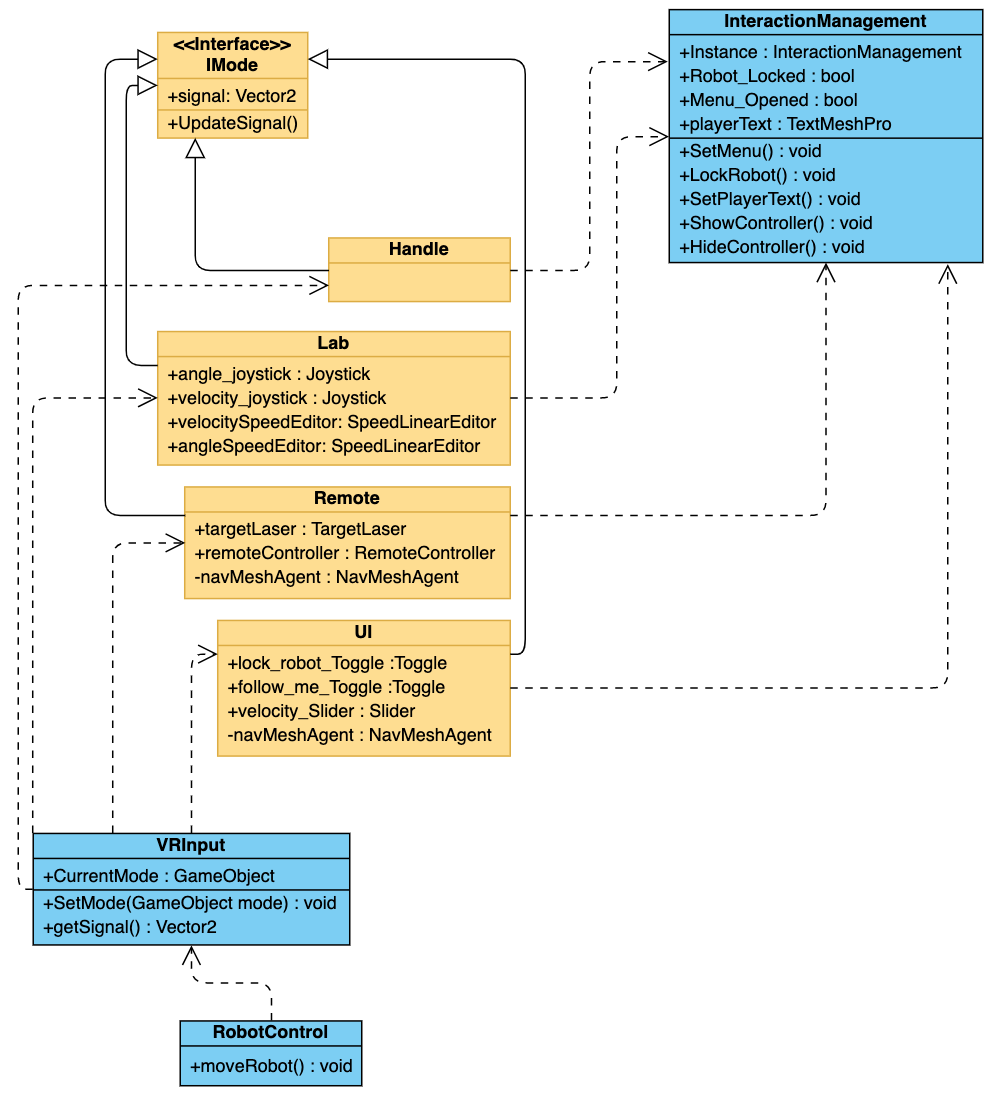
\includegraphics[height=12cm]{graphics/uml.png}
    \caption{UML Class diagram for the main structure of the system}
    \label{fig:uml}
\end{figure}

\subsection{Handle Mode}
\subsection{Lab Mode}
\subsection{Remote Mode}
\subsection{UI Mode}


\section{Test Scene}
In order to simulate the use of rescue robots in disaster scenarios, the test scenes were built to mimic the post-disaster urban environment as much as possible. The POLYGON Apocalypse\footnote{https://assetstore.unity.com/packages/3d/environments/urban/polygon-apocalypse-low-poly-3d-art-by-synty-154193}, available on the Unity Asset Store, is a low poly asset pack with a large number of models of buildings, streets, vehicles, etc. Using this resource pack as a base, additional collision bodies of the appropriate size were manually added to each building and obstacle after the pack was imported, which was needed to help track the robot's driving crash in subsequent tests.

Considering that there are four modes of operation to be tested, four scenes with similar complexity, similar composition of buildings but different road conditions and placement of buildings were constructed. The similarity in complexity of the scenes ensures that the difficulty of the four tests is basically identical. The different scene setups ensure that the scene information learned by the user after one test will not make him understand the next test scene and thus affect the accuracy of the test data. 

The entire scene is initially invisible, and the visibility of each objects in the test scene is gradually updated as the robot drives along. Ten interactable sufferer characters were placed in each test scene. The place of placement can be next to the car, the house side and some other reasonable places.

\chapter{Evaluation of User Experience}
\label{evaluate}

This chapter describes the design and detailed process of the user evaluation. The purpose of the performed user study is to measure the impact of four different operation modes on rescue efficiency, robot driving performance, and psychological and physiological stress and fatigue. For this purpose, participants are asked to find victims in a test scene using different operation modes and answer questionnaires after the test corresponding to each mode of operation.


\section{Study Design}

The evaluation for each operation mode consists of two main parts. The first part is the data recorded during the process of the participant driving the robot in the \gls{vr} environment to find the victims. The recorded data includes information about the robot's collision and the speed of driving etc. The rescue of the victims was also recorded. The second part is the questionnaires that participants filled out after each test. \gls{tlx} was used to measure the participant's subjective workload assessments. Additionally, participants were asked specific questions for each mode and were asked to select their favorite and least favorite operation mode. In order to reduce the influence of order effects on the test results, the Balanced Latin Square was used when arranging the test order for the four operation modes.



\section{Procedure}
\subsection{Demographics and Introduction }
Before the beginning of the actual testing process, participants were informed of the purpose of this work, the broad process and the content of data that would be collected. After filling in the basic demographics and signing a consent form, the features of each of the four modes of operation and their rough usage were introduced verbally with a display of the buttons on the motion controllers.



\subsection{Entering the world of VR}
After the essential introduction part, participants would put on the \gls{vr} headset and enter the \gls{vr} environment to complete the rest of the tutorial. Considering that participants might not have experience with \gls{vr} and that it would take time to learn how to operate the four different modes, the proposed system additionally sets up a practice pattern and places some models of victims in the practice scene. After entering the \gls{vr} world, participants first needed to familiarize themselves with the opening and closing menu, as well as using the motion controllers to try to teleport themselves, or raise themselves into mid-air. Finally, participants were asked to interact with the victim model through virtual hands. After this series of tutorials, participants were already generally familiar with the use of \gls{vr} and how to move around in the \gls{vr} world.



\subsection{Practice and evaluation of modes}
Given the different manipulation approaches for each mode and possible confusion between the different modes, participants would take turns practicing and directly evaluating each mode immediately afterward. 

The sequence of modes to be tested is predetermined. The order effect is an important factor affecting the test results. If the order of the operation modes to be tested would be the same for each participant, the psychological and physical exhaustion caused by the last operation mode would inevitably be more. In order to minimize the influence of the order effect on the results, the Balanced Latin Square with a size of four was used to arrange the test order of the four operation modes.

Participants automatically entered the practice scene corresponding to the relevant operation mode in the predefined order. After attempting to rescue 1-2 victims and when participants indicated that they were familiar enough with this operation mode, they would enter the test scene. In the test scene, participants had to save as many victims as possible in a given time limit. Participants were required to move the robot around the test scene to explore the post-disaster city and rescue victims. During this process, if the robot crashes with buildings or obstacles, besides the collision information being recorded as test data, participants would also receive sound and vibration feedback. The test would automatically end when time ran out or when all the victims on the scene have been rescued. Participants were required to complete the evaluation questionnaire and \gls{tlx} form at the end of each test. This process was repeated in each mode of operation. 

After all the tests were completed, participants were asked to compare the four operation modes and select the one they liked the most and the one they liked the least. In addition, participants could give their reasons for the choice and express their opinions as much as they wanted, such as suggestions for improvement or problems found during the operation.


\chapter{Conclusion}




\printbibliography

\end{document}
